% ============================================================================
\section{Classical synthesis}
% ============================================================================

\begin{frame}{Pre-2016 Era: Corpus-Based and Concatenative Synthesis}
  \begin{itemize}
    \item Early systems used \textbf{unit selection}: recording lots of speech from a single speaker and splitting it into small parts, usually syllables or \textbf{diphones}, a unit that runs from the middle of one phone to the middle of the next, so the hard part (the transition between two sounds) sits inside the recording rather than at a join.
    \item During synthesis, an algorithm picks which units to use by balancing:
    \begin{itemize}
      \item \textbf{Target cost} (how well each piece matches the desired sound)
      \item \textbf{Join cost} (how smooth the pieces sound when joined together)
    \end{itemize}
    \item This gives good local naturalness, but is not very flexible and can sound glitchy if needed transitions are missing from the database.
  \end{itemize}
\end{frame}

\begin{frame}{Statistical Parametric Synthesis}
  \begin{itemize}
    \item Statistical Parametric Speech Synthesis (SPSS) mainly used HMMs to model speech features instead of storing raw audio.
    \item SPSS models capture the spectral envelope, fundamental frequency ($F_0$), and duration of speech segments.
    \item Speaker adaptation is possible by updating a pre-trained model with a small amount of new speaker data, using maximum a posteriori (MAP) estimation or linear regression techniques.
    \item Trajectory HMMs were introduced to make transitions between features smoother and output speech more natural.
  \end{itemize}
\end{frame}

\begin{frame}{The HMM-based synthesis pipeline}
  \centering
  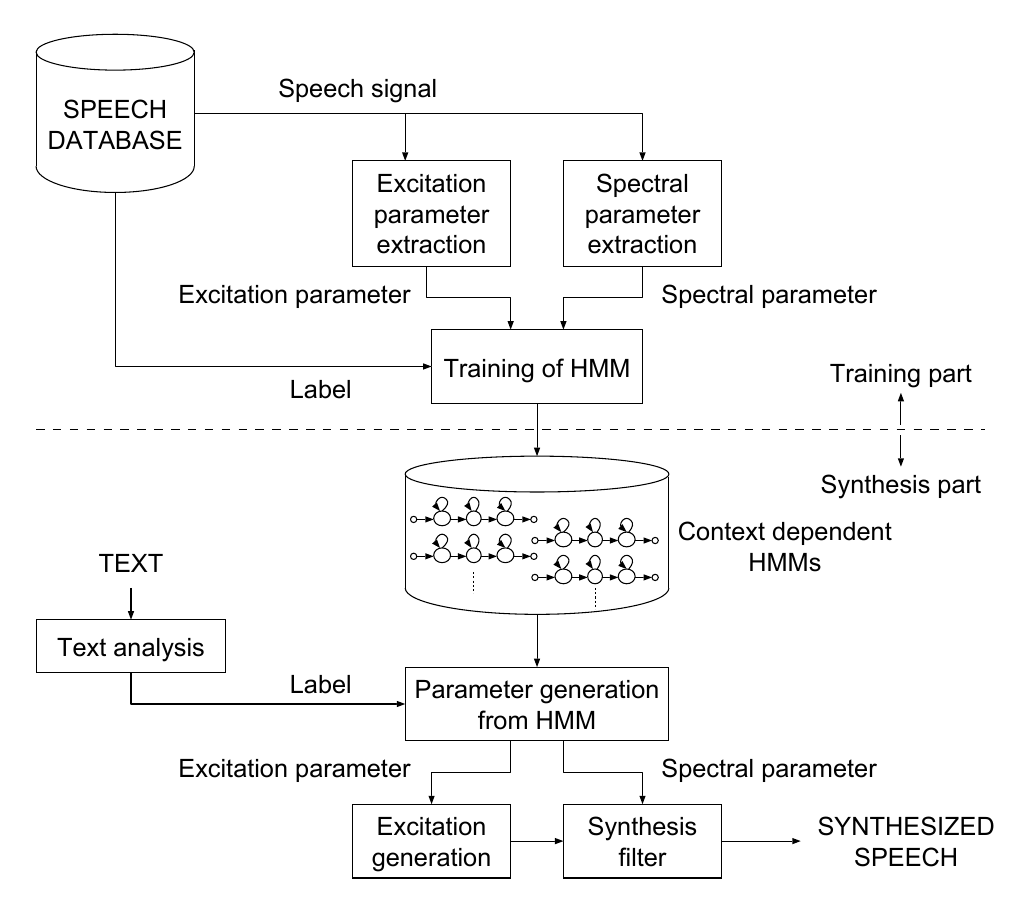
\includegraphics[width=\textwidth,height=0.76\textheight,keepaspectratio]{images/tts/hmm_spss_pipeline_tokuda_fig1.png}
  \slideimgsource{Tokuda, Zen \& Black, ``An HMM-Based Speech Synthesis System Applied to English,'' IEEE Workshop on Speech Synthesis, 2002, Fig.~1.}
\end{frame}
